\subsection{Separability of data} \label{sec:dataValidation}

%collect data (described earlier)
%review data to evaluate if the acquired data is valid for training the regressors
%do PCA to validate data (qualitatively) -> t-test (only later if we are fast) to check if data clouds are significalnty different from each other
%if data is different: good. if data not different: bad, redo data acquisition
%do training of regressors (next section)

After features has been extracted from the data, the feature data is validated through Principal Component Analysis (PCA) to determine the quality of the recorded data, to identify outliers and examining whether the data from the different hand gestures are distinguishable. Thus, the PCA is used as a qualitative tool to validate the data. %due to lack of time
%include if we are fast
%and t-test to decide if there are any significant outliers and if the features are significantly different from feature data of other movements. The PCA is used to determine the relation between the feature data and identifying data outliers. 
%What is PCA?
PCA is an analysis tool used to express a set of correlated variables into non-correlated components, such that the dataset can be expressed in a reduced dimensionality hyperspace using less variables, however more defining variables for the given data set. These variables are called the principal components. Each principal component is orthogonal on the former, meaning that they each define the largest variance in an axis, different from axes described by other components. PCA also provides knowledge on which components are the most defining for the dataset, where the first vectors in the hyperspace being the ones with highest variance, so only the most important can be considered. 

When performing PCA it provides the most defining values of the data. The most defining values are determined by a 90\% threshold for the principal components. This means that only the principal components who account for describing the first 90\% of the data will be included in further work. The data described by the used principal components can be visualised in a three dimensional plot. In the setting of this project it can be used to determine the separability of the data and thus the quality of the data. If the data proves to be distinguishable it will be clustered in clouds separate from each other. If the data clouds are mixed and overlaps, the data is not separable and thus of poor quality. 

%coefficients of the principal components (PCC), which can be visualised in a plot. This plotting of the coefficients are what is used to evaluate the quality of the feature data. A threshold of 90\% for preserved information is used.

PCA is performed for each movement in each limb position and plotted in a three dimensional space. The result of the PCA will determine the quality of the recorded data. If there exist significant outliers a new recording session for the test subject can be executed to prevent inaccurate training of regressors and time delays. If the data is clustered and easily distinguishable from each other, it can be used further on to train the regressors.


% MOVED TO RESULTS
%
%\begin{figure}[H]
%	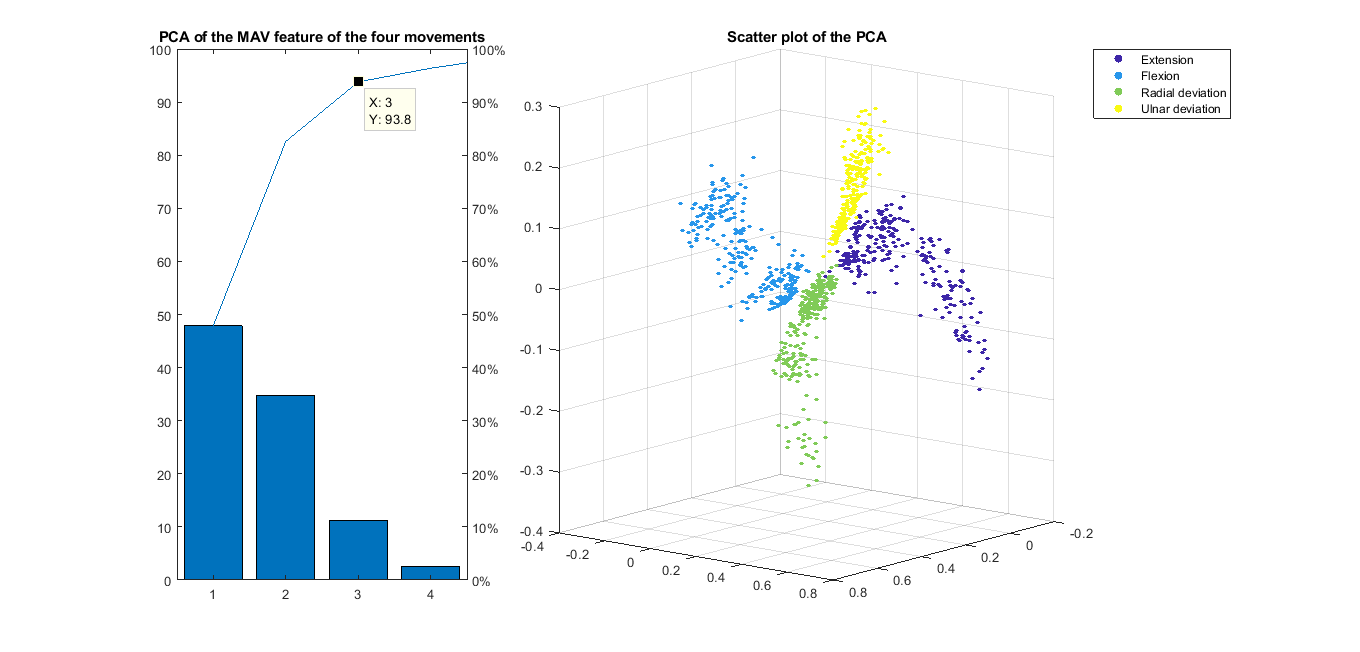
\includegraphics[width=1\textwidth]{figures/Methods/pcasubplot.png} 
%	\caption{Plot of PCA. To the left the first four principal components are visualised. The first three principal components account for describing $93.8\%$ of the data set. On the right the PCC's are plotted for each movement. The clusters for each movement are distinguishable from each other and have no noteworthy outliers, so the data is considered of high quality.} 
%	\label{fig:pcasubplot}
%\end{figure} 
%
%In \figref{fig:pcasubplot} an example of a PCA performed on feature data from one test subject is shown. The left plot of the principal components describe the importance of each identified components, and how much of the variance in the data that is described. Using only the first three components, $93.8\%$ of the full dataset can be described. Only these principal components are used in the plot to the right in \figref{fig:pcasubplot}. Here it can be seen that the clusters are easily distinguishable and have no remarkable outliers. Therefore the data is considered good and can be used in the training of the regressors.





